\section{Selecting curated Workflows}

%%%%%%%%%%%%%%%%%%%%%%%%%%%%%%%%%%%%%%%%%%%%%%%%%%%%%%%%%%%%%%%%%%%%%%%%%%%%%%%%
\begin{frame}
    \frametitle{Outline}
    \begin{columns}[t]
        \begin{column}{.5\textwidth}
            \tableofcontents[sections={1-9},currentsection]
        \end{column}
        \begin{column}{.5\textwidth}
            \tableofcontents[sections={10-18},currentsection]
        \end{column}
    \end{columns}
\end{frame}

%%%%%%%%%%%%%%%%%%%%%%%%%%%%%%%%%%%%%%%%%%%%%%%%%%%%%%%%%%%%%%%%%%%%%%%%%%%%%%%%
\begin{frame}
  \frametitle{What is this about?}
   \begin{question}[Questions]
   	 \begin{itemize}
       \item How do I get a workflow for a given scientific problem?
       \item How do I run such an arbitrary workflow?
     \end{itemize}
   \end{question} 
   \begin{docs}[Objectives]
   	  \begin{enumerate}
                      \item Introducing the worfkflow catalogue?
                      \item Learning the difference between ``curation'' (what some people think) and ``curation'' (what really works)?
      \end{enumerate}
    \end{docs}
\end{frame}  

\subsection{The \texttt{Snakemake} Workflow Catalogue}

%%%%%%%%%%%%%%%%%%%%%%%%%%%%%%%%%%%%%%%%%%%%%%%%%%%%%%%%%%%%%%%%%%%%%%%%%%%%%%%
\begin{frame}
 \frametitle{Selecting and Downloading from the Workflow Catalogue}
 You can find the \texttt{Snakemake} worfkflow catalogue, \lhref{https://snakemake.github.io/snakemake-workflow-catalog/?rules=true}{here}. It makes a difference between workflows which meet best-practice criteria - and those which do not.\newline
 \begin{columns}
   \begin{column}{0.5\textwidth}
     You can download and run any workflow. \pause\newline
     \begin{warning}
     	Except, you most likely cannot, because of a missing cluster configuration and some missing features.
     \end{warning}
   \end{column}
   \begin{column}{0.5\textwidth}
     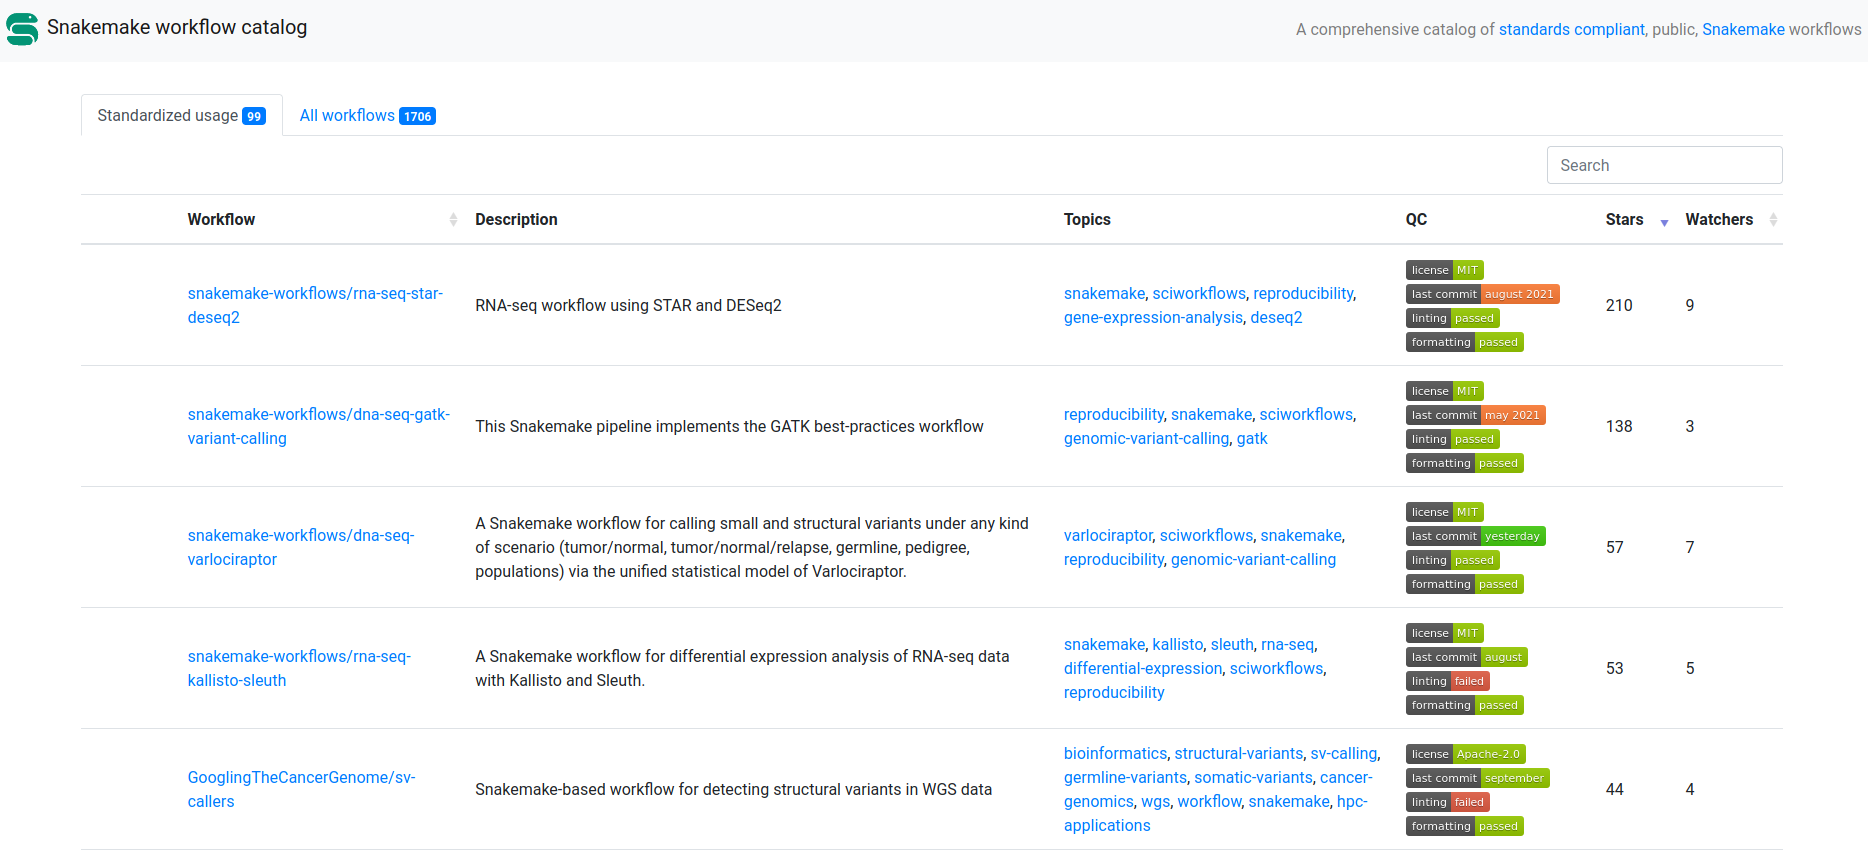
\includegraphics[width=\textwidth]{Snakemake/Snakemake_Workflow_Catalog.png}
   \end{column}
 \end{columns}
\end{frame}

%%%%%%%%%%%%%%%%%%%%%%%%%%%%%%%%%%%%%%%%%%%%%%%%%%%%%%%%%%%%%%%%%%%%%%%%%%%%%%%%
\begin{frame}[fragile]
  \frametitle{Deployment}
  Select (=click on) any desired workflow. There are two alternatives:
  \begin{enumerate}
   \item a workflow offers a release - in which case you can download and unpack it
   \item all workflows offers a ``\altverb{git clone}'' hint
  \end{enumerate}
\end{frame}

%%%%%%%%%%%%%%%%%%%%%%%%%%%%%%%%%%%%%%%%%%%%%%%%%%%%%%%%%%%%%%%%%%%%%%%%%%%%%%%%
\begin{frame}[fragile]
  \frametitle{Running Workflows on Cluster (or other environment)}
  Most likely a specific workflow never has been testing on \emph{your} computer before. It is almost ensured it will run on arbitrary servers, but clusters are a different story. \newline
  So
  \begin{itemize}[<+->]
   \item try to parameterize your workflow as learned
   \item if it gives issues and you know how to correct it, ``fork'' the worklow and create a pull request
   \item if you cannot fix it, create a bug report
  \end{itemize}
\end{frame}

%%%%%%%%%%%%%%%%%%%%%%%%%%%%%%%%%%%%%%%%%%%%%%%%%%%%%%%%%%%%%%%%%%%%%%%%%%%%%%%%
\begin{frame}
  \frametitle{\Interlude{Learn git!}}
  If you do not know what ``fork'' and ``pull request'' means, learn git!
  \begin{itemize}[<+->]
   \item there are courses
   \item and lots of online material
   \item and books
  \end{itemize}
  \pause
  \begin{warning}
  	Knowing git is essential in data analysis!
  \end{warning}
\end{frame}


